\section{Additional Exploratory Diagnostics}
\label{app:exploratory}
The following plots describe the frozen 36-landmark confirmation set. They do not alter the calibrated settings. Percentages in Figure~\ref{fig:all-landmarks} are per-landmark changes. Main-text aggregate percentages are ratios of cohort means. No tested association survives global correction over 46 primary exploratory tests.

\begin{figure}[htbp]
\centering
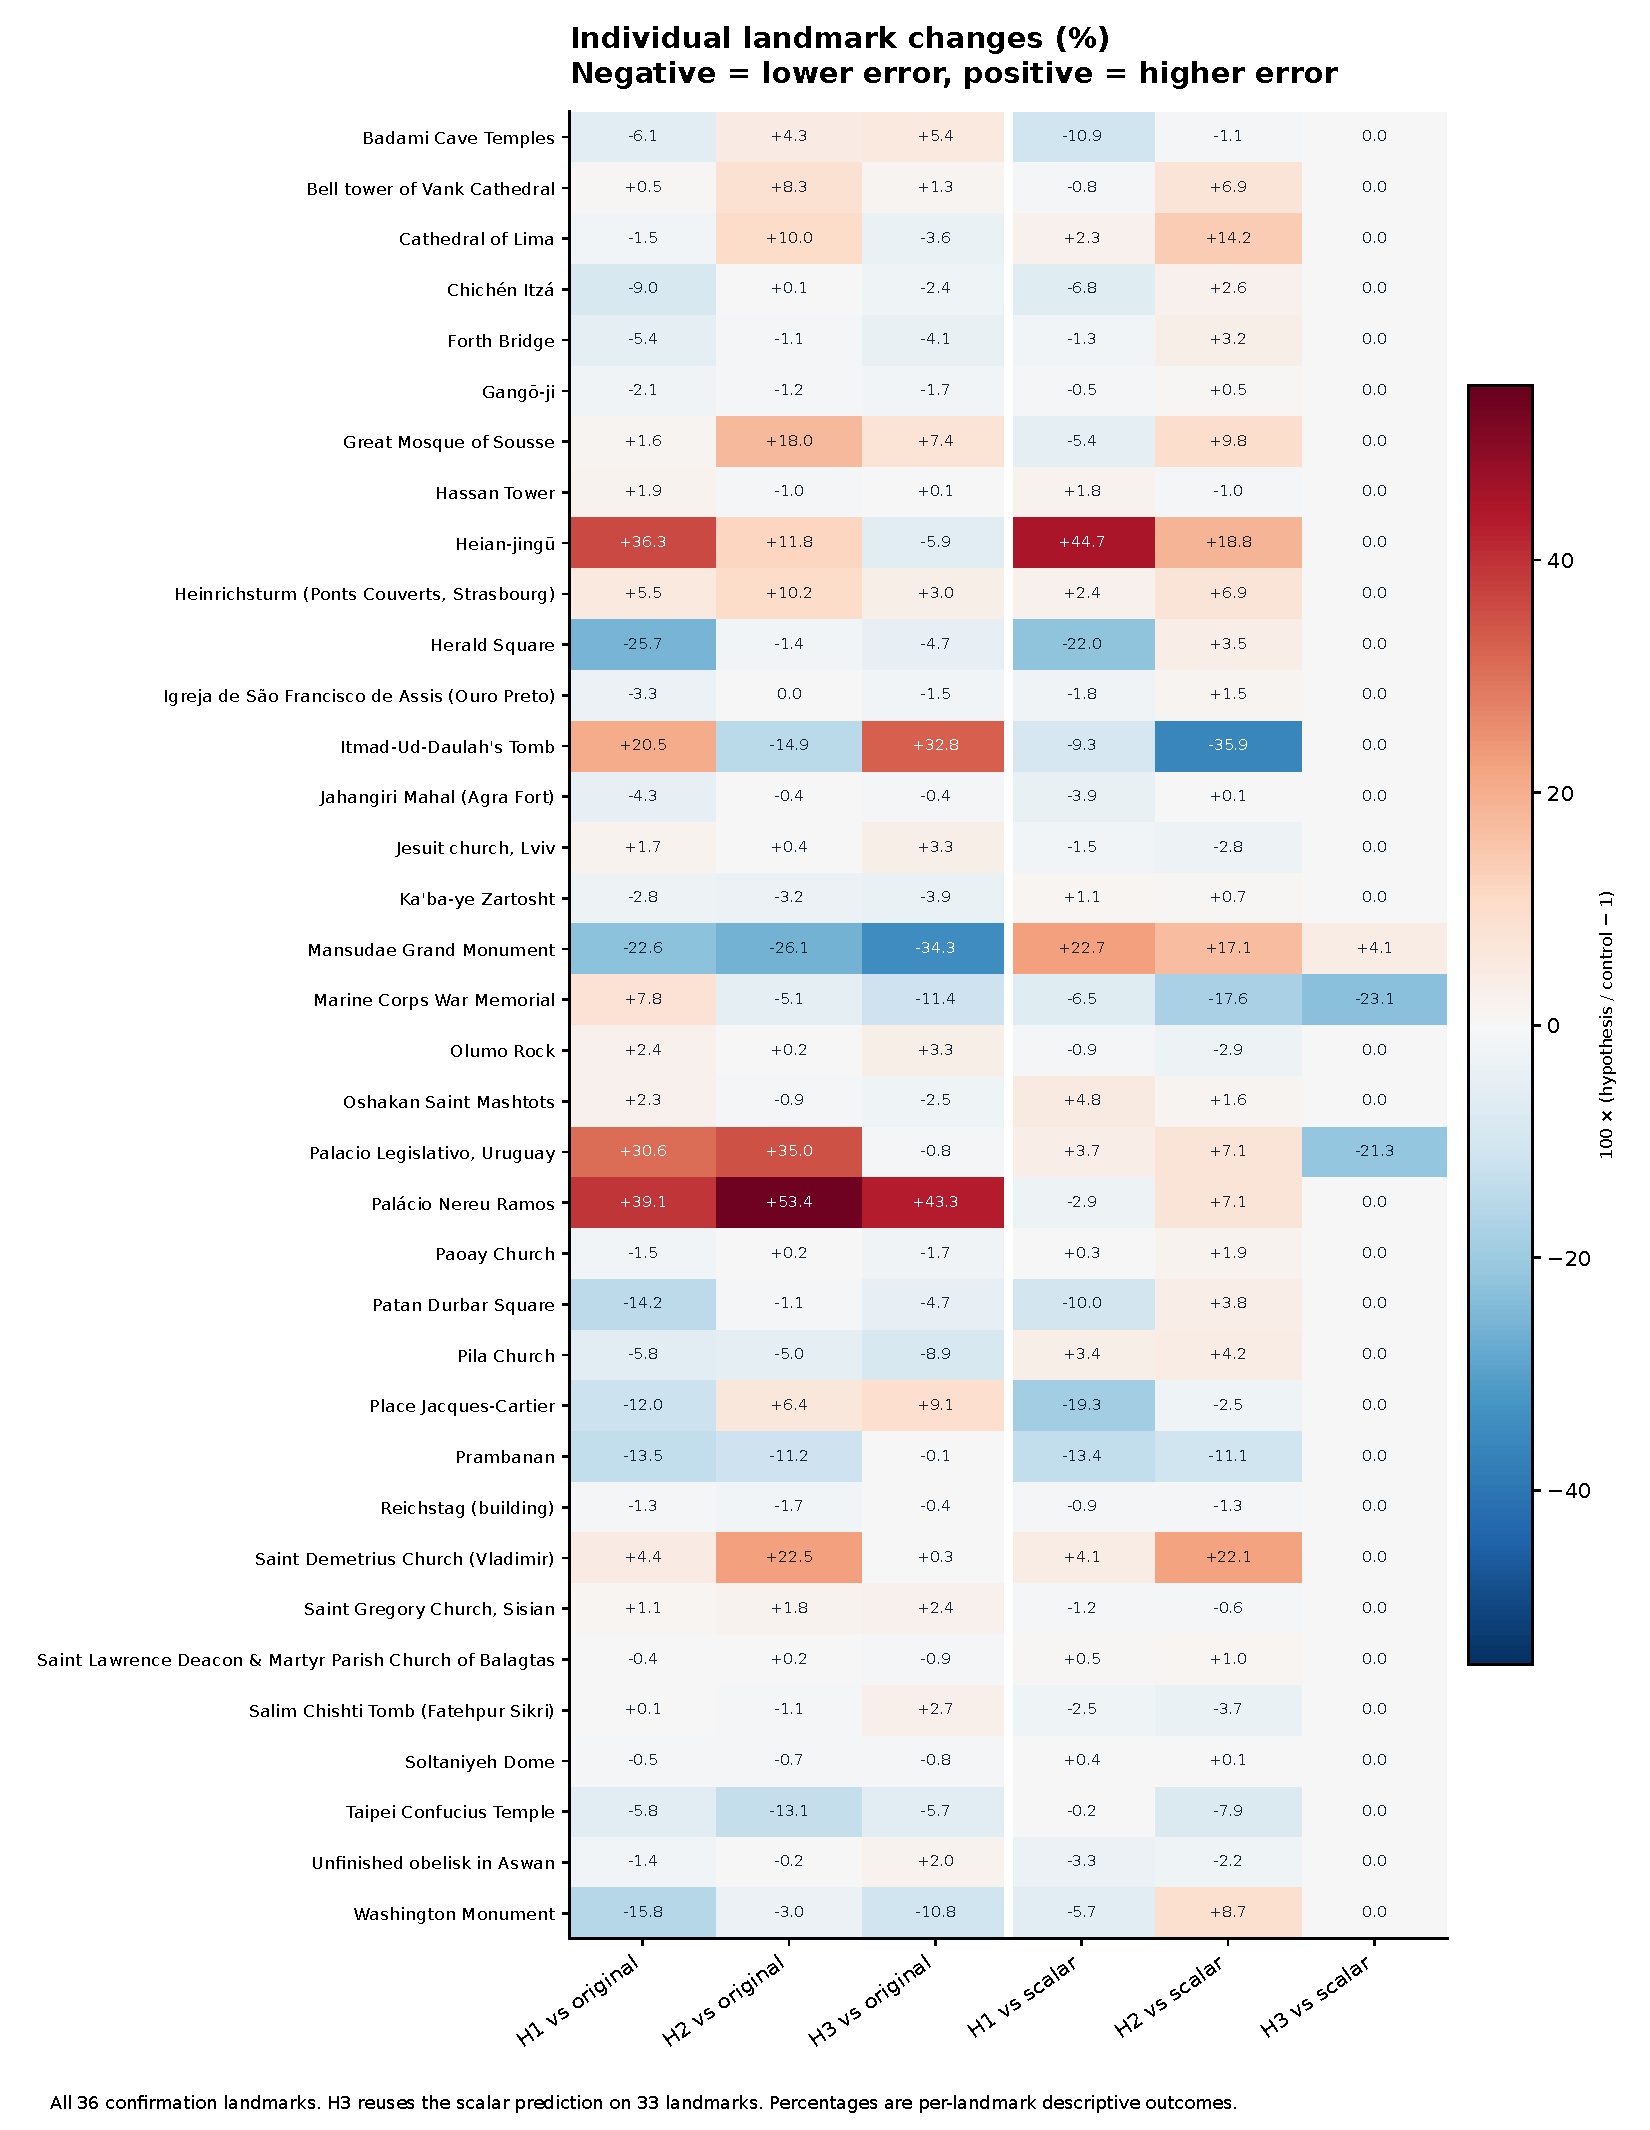
\includegraphics[width=0.86\textwidth,height=0.76\textheight,keepaspectratio]{figures/extended_landmark_changes.pdf}
\caption{All 36 confirmation landmarks and both comparators. Negative percentage changes are improvements. The full matrix retains failures and the 33 exact H3--scalar ties.}
\Description{A heatmap shows all landmark percentage changes for H1, H2, and H3 against original and scalar predictions.}
\label{fig:all-landmarks}
\end{figure}
\clearpage
\begin{figure}[htbp]
\centering
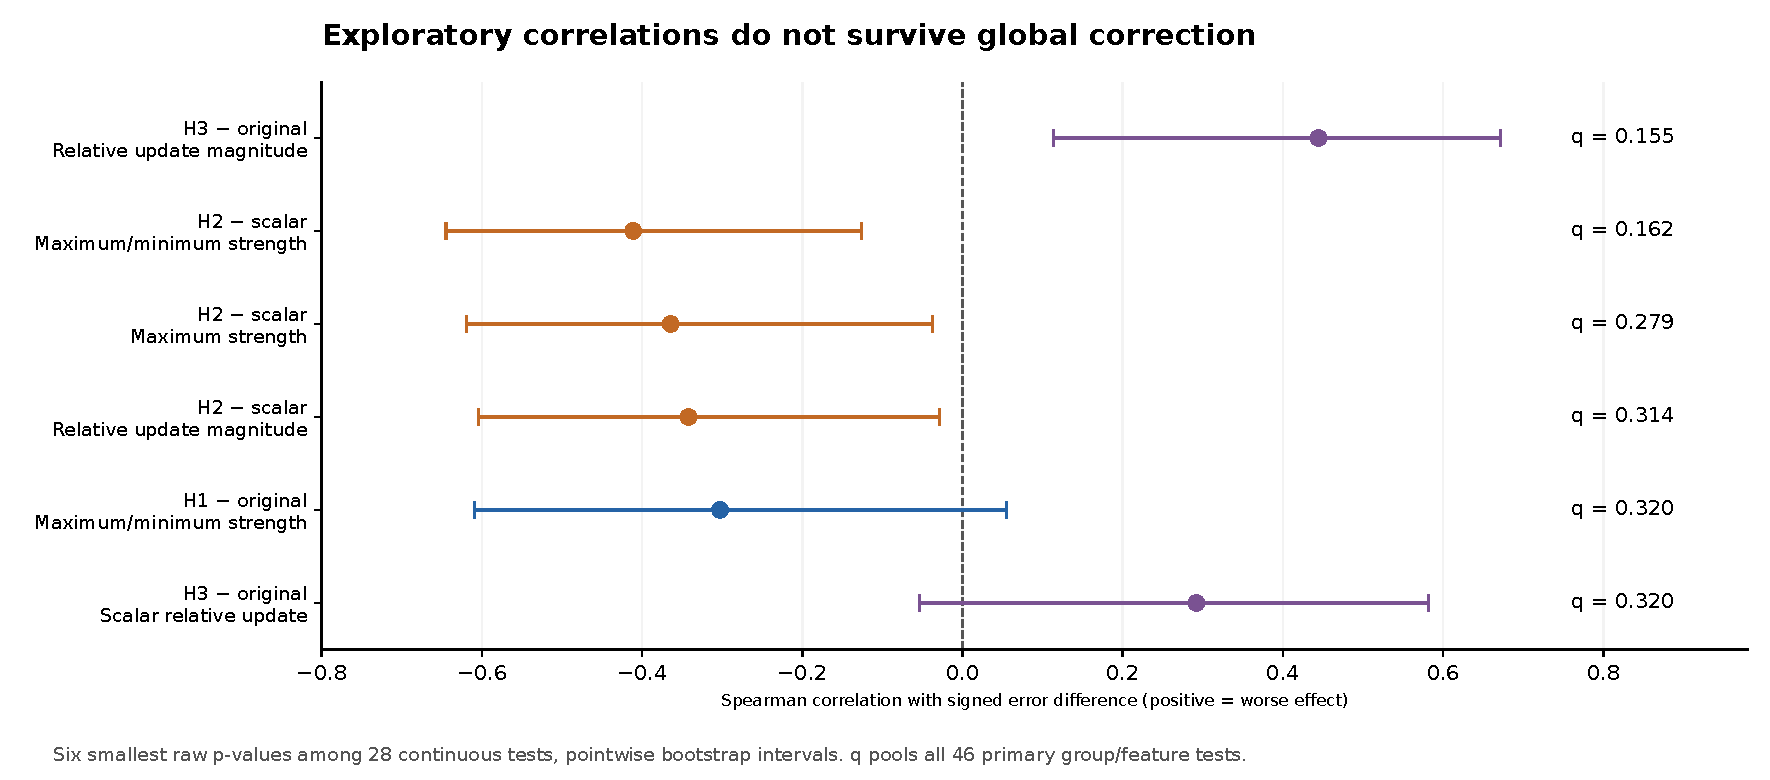
\includegraphics[width=\textwidth]{figures/extended_exploratory_correlations.pdf}
\caption{The six strongest primary continuous-feature associations by uncorrected evidence. Labels report the global BH correction over 46 tests. The complete result table, including nonsignificant associations, is included in \nolinkurl{extended_evidence/all_exploratory_primary_tests.csv}.}
\Description{Six exploratory rank correlations and their intervals, none passing correction across the complete search.}
\end{figure}
\begin{figure}[htbp]
\centering
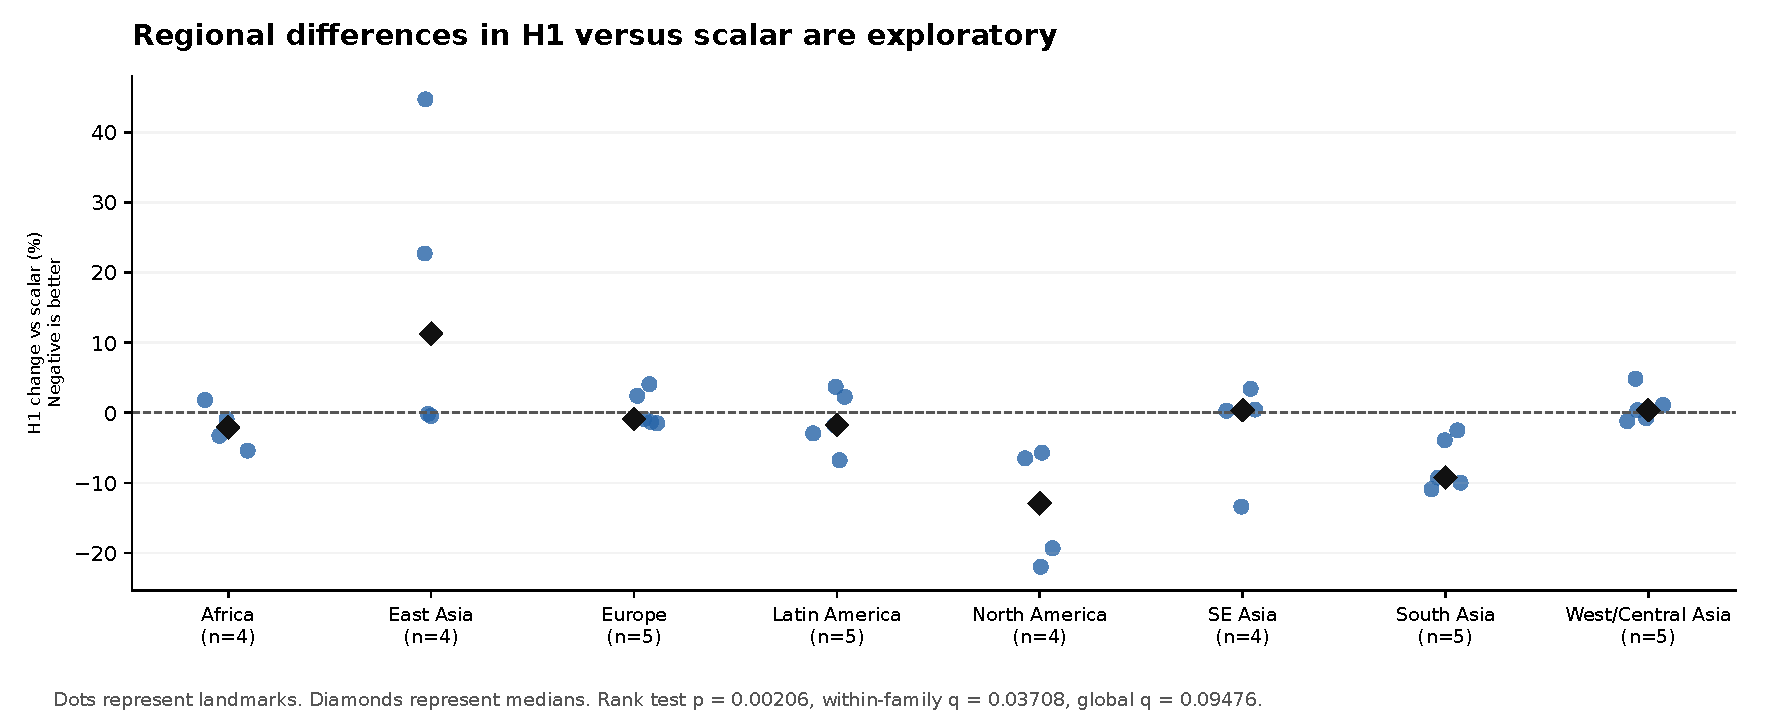
\includegraphics[width=\textwidth]{figures/extended_h1_regional_pattern.pdf}
\caption{Individual H1 percentage changes relative to the scalar, grouped by region. Markers summarize the distributions with medians. The formal omnibus test is rank-based and does not test the plotted medians directly. Small group sizes and overlapping scene attributes limit interpretation.}
\Description{Regional groups of individual H1 changes relative to the scalar, showing both improvements and regressions.}
\end{figure}
\clearpage
